%%%%%%%%%%%%%%%%%%%%%%%%%%%%%%%%%%%%%%%%%%%%%%%%%%%%%%%%%%%%%%%%%%%%%%%%%%%%%%%%
% experiment.tex: Chapter describing the experiment
%%%%%%%%%%%%%%%%%%%%%%%%%%%%%%%%%%%%%%%%%%%%%%%%%%%%%%%%%%%%%%%%%%%%%%%%%%%%%%%%
\chapter{Heavy Photon Search}
\label{chapter:hps:experiment}

\acf{hps} is a fixed-target experiment currently in operation at \ac{jlab}
which is focused on search for short-length (few centimeter) decays of new particles.
In order to search for these visible signatures of new particles,
\ac{hps} must be able to precisely reconstruct the produced \ac{sm} particle
kinematics and then use this information to estimate their origin point (their
``vertex'').
This reconstruction is enabled by two key detector components whose design
will be motivated using the model studied in more detail in this part.

\section{Strongly Interacting Massive Particles}
\label{sec:hps:simps}

As mentioned in \cref{sec:theory:visible}, our search for \ac{dm} must accomodate the possibility
that any \ac{dm} produced within our experiments subsequently decays back into \ac{sm} particles.
In order to model these types of \ac{dm}, we must account for both how the \ac{dm} is produced and
how it decays back to \ac{sm} particles. These theories propose new specific vertex rules for
constructing the Feynman diagrams and for the vertex factors within the calculations.

To be even more specific, we could hypothesize that the dark sector consists of particles that
interact with each other strongly in the same sense of the standard quarks. These Strongly
Interacting Massive Particles (SIMPs) \cite{simp-mechanism-2014,simp-pheno-2018} would then form
composite particles similar to how standard quarks form composite particles like protons and
neutrons. Since we expect our experiments to not reach the energies required to separate the
constiuents of these composite particles, the composite particles themselves would be the dark
matter candidates and the ones we represent within our diagrams. A dark sector consisting of SIMPs
would have a plethora of composite particles which we could observe; however of particular
importance is that there could be a composite particle that has similar enough properties to the
dark photon that it could ``mix'' with it and decay in a way that emits fewer dark particles:
\cref{fig:dark-brem-simp-decay}. This decay, since it has less energy ``lost'' to the dark
particles, has a greater potential of being observed within \ac{hps} and is discussed here.

\begin{figure}
  \centering
  \begin{tikzpicture}
  \begin{feynman}
    \vertex (a) {$e^{-}$};
    \vertex [right= of a](d);
    \vertex [below=of d, blob,label={below:$Z$}] (e) {};
    \vertex [right= of d] (b);
    \vertex [above right= of b] (g) {$e^{-}$};
    \vertex [below right= of b] (aprime_decay);
    \vertex [below right= of aprime_decay] (rhod_decay);
    \vertex [above right= of aprime_decay] (dm) {$\pi_D$};
    \vertex [below right= of rhod_decay] (i);
    \vertex [above right= of i] (j) {$e^{-}$};
    \vertex [below right= of i] (k) {$e^{+}$};
    \diagram*[large] {
    (a) -- [fermion] (d),
    (d) -- [boson] (e),
    (d) -- [fermion] (b),
    (b) -- [fermion] (g),
    (b) -- [boson, edge label={$A'$}] (aprime_decay) -- [double, edge label={$V_D$}] (rhod_decay),
    (aprime_decay) -- [scalar] (dm),
    (rhod_decay) -- [boson, edge label={$A'^*$}] (i),
    (k) -- [fermion] (i) -- [fermion] (j),
    };
  \end{feynman}

  \node [below=of e,align=left] (param)
    {\(\frac{m_{A'}}{m_{V_D}} = \frac{5}{3}\quad\frac{m_{A'}}{m_{\pi_D}} = 3\)\\%
    \(\frac{m_{\pi_D}}{f_{\pi_D}} = 4\pi\quad\alpha_D = 0.01\)};
\end{tikzpicture}

  \caption{
    Diagram of dark brem production of a dark photon followed by its decay back into an electron-positron pair
    through SIMP composite particle $V_D$ with the emission of a lighter SIMP composite particle $\pi_D$.
    The two-particle vertex $V_D-A'$ is only allowed since they share enough quantum properties to mix.
  }
  \label{fig:dark-brem-simp-decay}
\end{figure}

Importantly, \cref{fig:dark-brem-simp-decay} has two vertices where \ac{dm} and \ac{sm} particles
interact -- these two vertices represent the fact that such a visible decay is subsequently less
probable since both of these vertices carry with them the weak mixing factor $\epsilon$. The lower
probability of these visible decays is a general property of such signatures and motivates
experiments focused on collecting large data volumes in order to overcome the limitation imposed by
this lower probability. With this in mind, \ac{hps} has been built to observe a beam whose rate is
significantly high -- high enough to prevent sensitive detector elements from being placed directly
within its path.

The observable outgoing particles of \cref{fig:dark-brem-simp-decay} can be mimiced by existing
\ac{sm} processes. The most prominent background process is trident production \cref{fig:trident}
which enables the production of the electron-positron pair through the radiation of the virtual
photon (\cref{fig:trident:radiative}) or through direct electromagnetic interaction with the
nucleus and a virtual lepton (\cref{fig:trident:bethe-heitler}). The upside of this trident
production process is that it is \emph{prompt} -- i.e. the produced electron and positron originate
from within the target. The position of this vertex is a separation from the signal process
\cref{fig:dark-brem-simp-decay} where the vertex of the produced electron and positron would be
observably displaced downstream of the target due to the non-zero lifetime of the dark sector
particle $V_D$.

\begin{figure}
  \centering
  \begin{subfigure}[t]{0.4\textwidth}
    \begin{tikzpicture}
      \begin{feynman}
        \vertex (a) {$e^{-}$};
        \vertex [right= of a](d);
        \vertex [below=of d, blob,label={below:$Z$}] (e) {};
        \vertex [right= of d] (b);
        \vertex [above right= of b] (g) {$e^{-}$};
        \vertex [below right= of b] (rad);
        \vertex [above right= of rad] (j) {$e^{-}$};
        \vertex [below right= of rad] (k) {$e^{+}$};
        \diagram*[large] {
        (a) -- [fermion] (d),
        (d) -- [boson] (e),
        (d) -- [fermion] (b),
        (b) -- [fermion] (g),
        (b) -- [boson, edge label={\(\gamma^*\)}] (rad),
        (k) -- [fermion] (rad) -- [fermion] (j),
        };
      \end{feynman}
    \end{tikzpicture}
    \caption{Radiative trident}
    \label{fig:trident:radiative}
  \end{subfigure}%
  ~
  \begin{subfigure}[t]{0.4\textwidth}
    \begin{tikzpicture}
      \begin{feynman}
        \vertex (a) {$e^{-}$};
        \vertex [right= of a] (d);
        \vertex [above right= of d] (g) {$e^{-}$};
        \vertex [below right=of d] (eleprod);
        \vertex [below=of eleprod] (posprod);
        \vertex [right=of eleprod] (j) {$e^{-}$};
        \vertex [right=of posprod] (k) {$e^{+}$};
        \vertex [below left=of posprod, blob,label={below:$Z$}] (e) {};
        \diagram*[large] {
        (a) -- [fermion] (d) -- [fermion] (g),
        (d) -- [boson] (eleprod),
        (e) -- [boson] (posprod),
        (k) -- [fermion] (posprod) -- [fermion] (eleprod) -- [fermion] (j),
        };
      \end{feynman}
    \end{tikzpicture}
    \caption{Bethe-Heitler trident}
    \label{fig:trident:bethe-heitler}
  \end{subfigure}
  \caption{Feynman diagrams for the \ac{sm} process of trident production.}
  \label{fig:trident}
\end{figure}

\ac{hps} is designed to focus on visible signatures of \ac{dm} like SIMPs with
a dual strategy of searching for mass resonances and displaced vertices.
Both of these strategies require high data volume and precise reconstruction of a produced
electron-positron pair originating from the decay of some \ac{dm} particle.
The precision of this reconstruction is one of the main limiting factors in distinguishing
whether a specific pair originated from \ac{dm} or from some other \ac{sm} background process.
These design drivers have led to the the apparatus discussed below.

\section{Detector Apparatus}
%%%%%%%%%%%%%%%%%%%%%%%%%%%%%%%%%%%%%%%%%%%%%%%%%%%%%%%%%%%%%%%%%%%%%%%%%%%%%%%%
\ac{hps} is currently installed behind the CLAS-12 experiment in the Hall B
alcove at \ac{jlab} and utilizes the \ac{cebaf} to provide its beam
\cite{mrsolt-thesis-2020,skmccarty-thesis-2020}.
Hall B primarily hosts the CLAS-12 experiment in the bulk of its hall; nevertheless,
behind the CLAS-12 experiment \ac{hps} is situated
within an alcove such that it can collect data whenever CLAS-12 is not operational (for example,
when its components are being upgraded or fixed).

\ac{cebaf} \cite{cebaf-12GeV-2012,cebaf-opportunities-2012,cebaf-2013} is able to
provide a near-continuous electron beam ranging in energy up to $12$ GeV in steps
of $\approx 1.15$ GeV. \ac{cebaf} is built in a oval ``race track'' where the straight
portions consist of linear accelerators and the curve portions steer the beam with
dipole magnets either back into the straight portions or into experimental halls.
Since \ac{cebaf} delivers electrons at such a high rate, \ac{hps} must be able to
handle these high radiation loads. Designed to be a small experiment to fit within
the Hall B alcove, \ac{hps} elected to be built in two halves that straddle the primary
path of the beam where the highest amount of radiation would be. Both of the subsystems
within \ac{hps} are split into these two halves as shown in \cref{fig:hps-full-render}
and \cref{fig:hps-diagram}.

\begin{figure}
  \centering
  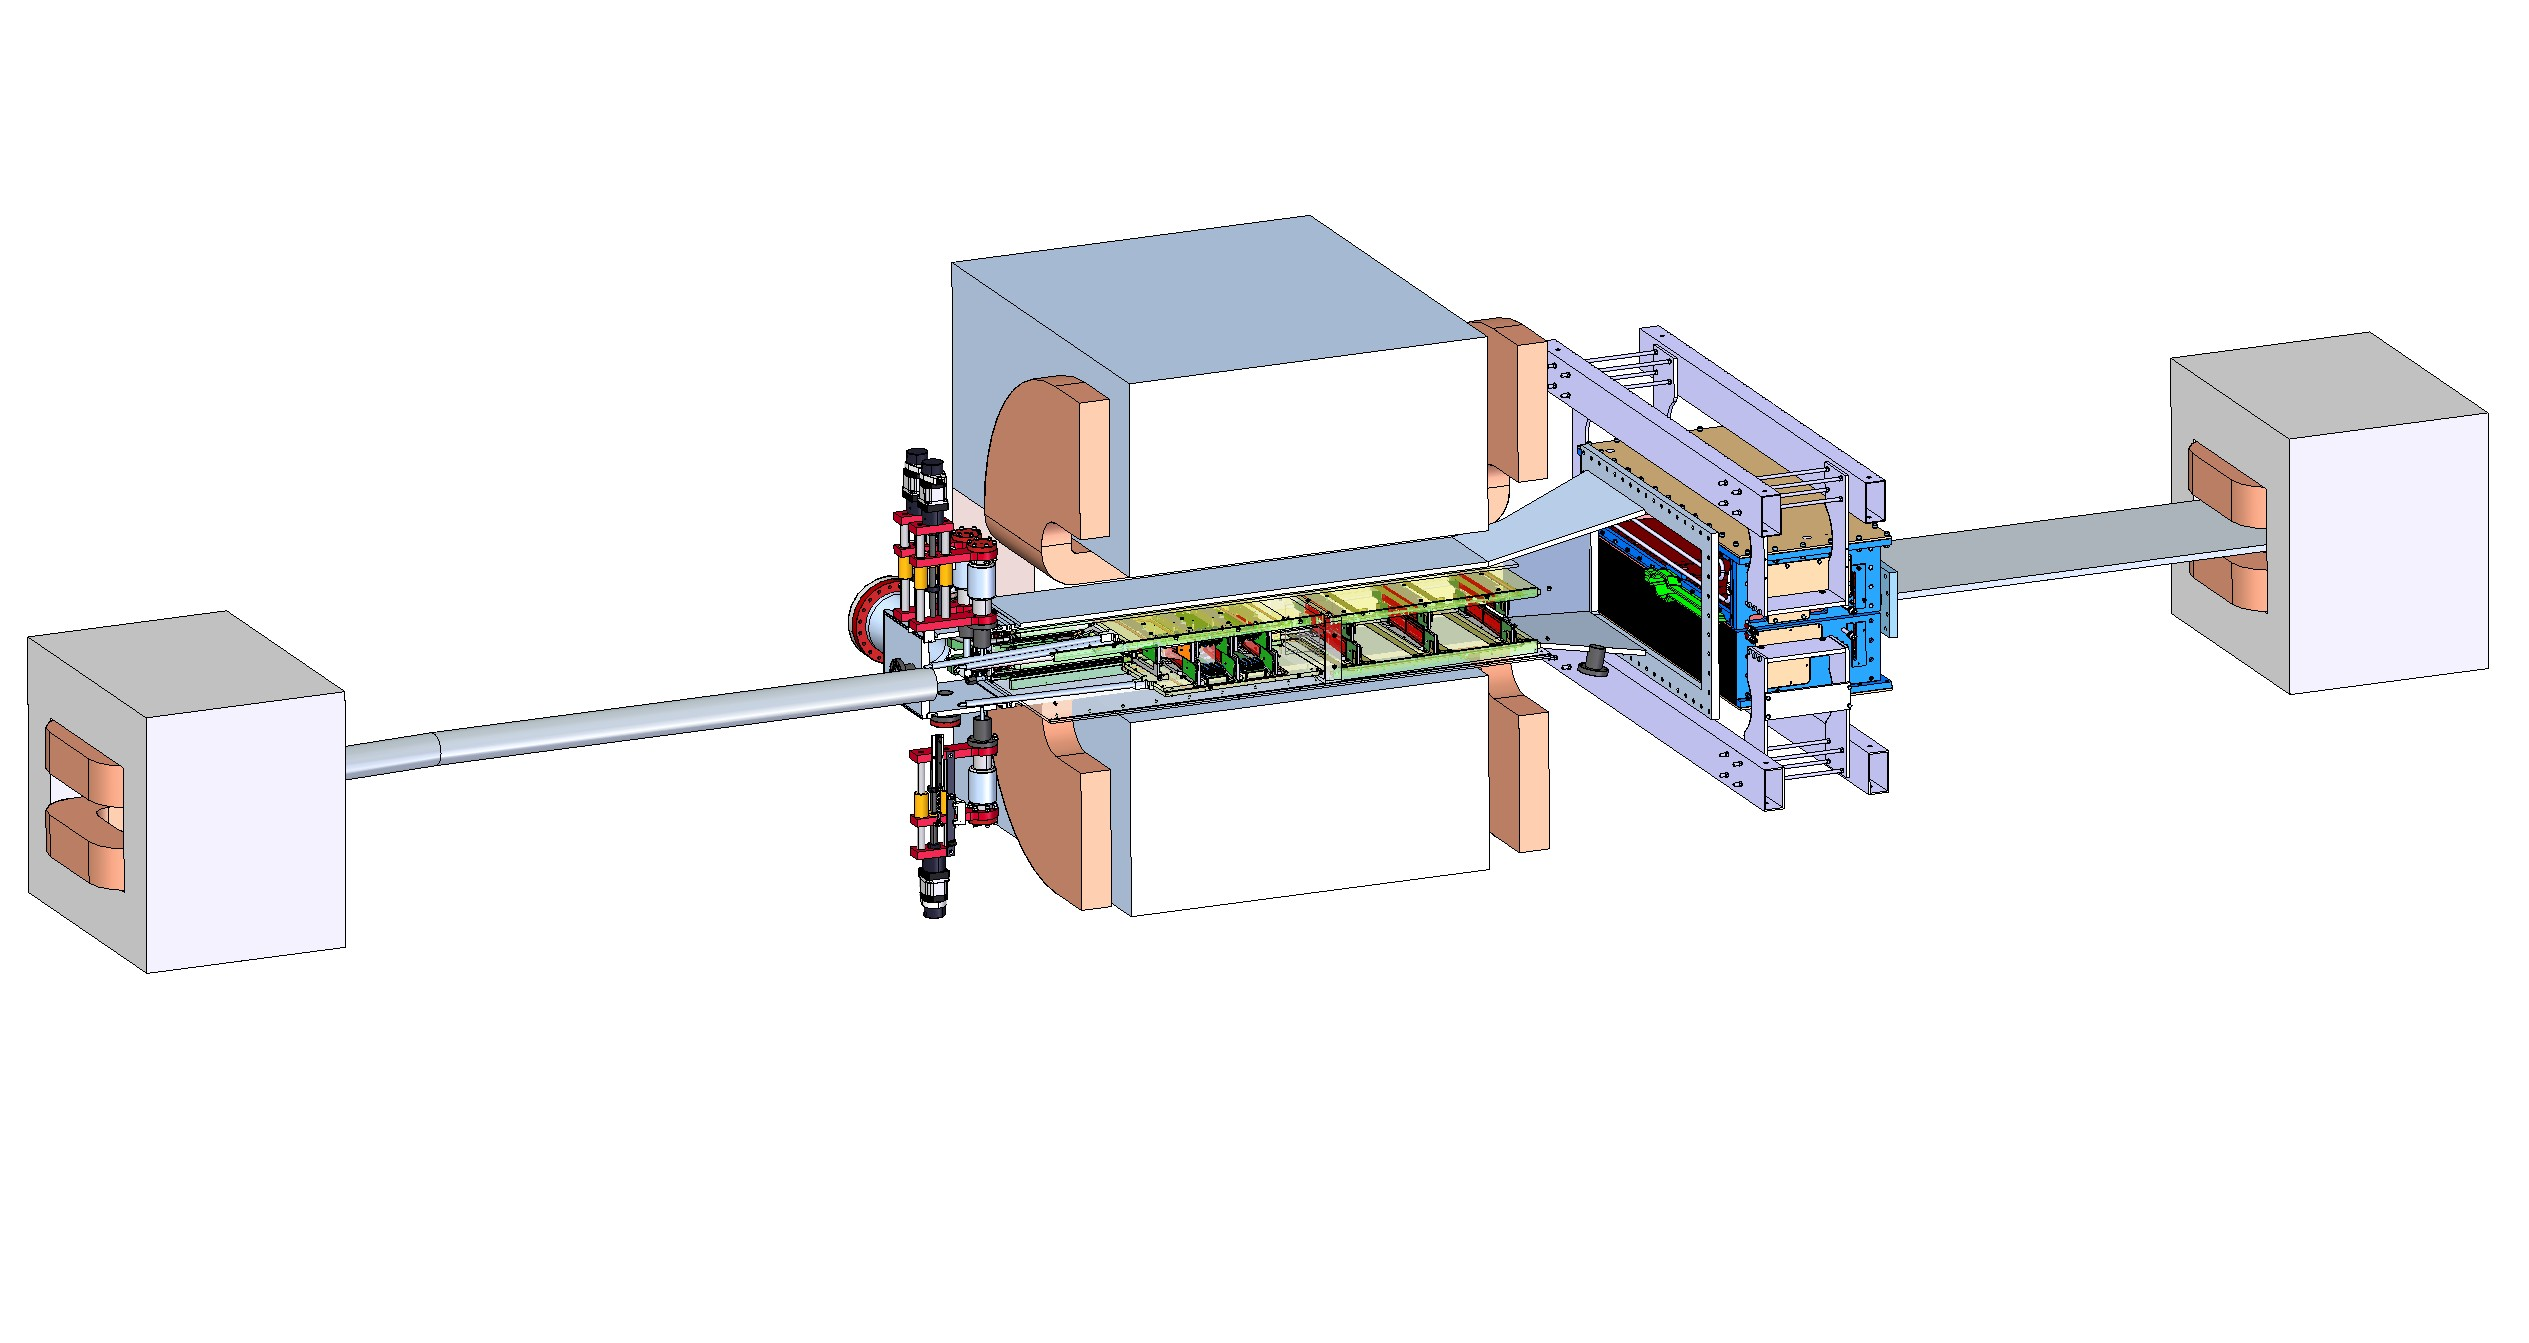
\includegraphics[trim={15cm 10cm 10cm 5cm},clip,width=\textwidth]{figures/hps/experiment/hps_full_render.jpg}
  \caption{
    Full rendering of \ac{hps}.
    Beam would enter the detector from the left and exit to the right if it does not interact.
  }
  \label{fig:hps-full-render}
\end{figure}

\begin{figure}
  \centering
  \resizebox{\textwidth}{!}{\begin{tikzpicture}
  \drawhps
\end{tikzpicture}
}
  \caption{
    Simplified diagram of \ac{hps} showing an example displaced decay within the named subsystems.
    The blue arrow is some \ac{dm} candidate particle that has a macroscopic lifetime causing
    the decay vertex to be observably displaced from the production within the target.
  }
  \label{fig:hps-diagram}
\end{figure}

The two subsystems included within \ac{hps} are the \ac{svt} focused on reconstruction of the
momentum and charge of charged particles and the \ac{ecal} focused on energy reconstruction and
online triggering of the data.

\subsection{Silicon Vertex Tracker}
The \ac{svt} is made of eighteen modules each of which is a pair of silicon-strip detectors offset
from each other by a small angle to enable three-dimensional position reconstruction. The modules
are arranged in the two halves separated by the center beam line. In each half, the modules are put
into layers with the first three layers consisting of one module while the last three layers
consisting of two modules to increase angular acceptance relative to the target.
\cref{fig:hps-svt-render} shows a rendering of the \ac{svt} with the sensitive detector elements
shown as red rectangles.\footnote{ This diagram and the description within this thesis is focused
  on the \ac{hps} \ac{svt} from its physics run in 2016. Various \ac{hps} components have been
  upgraded for subsequent runs. }

The two halves of the \ac{svt} are positioned to form a \qty{15}{\milli\radian} angular gap
relative to the target in order to avoid the largest amount of radiation from the beam. The first
layer (closest to the target, left size of \cref{fig:hps-svt-render}) is placed \qty{10}{\cm} from
the target and \qty{0.5}{\mm} from the beam line in order to maximize acceptance. The entire
\ac{svt} is enclosed in a vacuum box to limit secondary production of particles and is liquid
cooled to help prevent radiation damage.

The \ac{svt} modules are readout by APV25 chips which report six samples every \qty{24}{\ns}. These
samples are only dumped to disk upon receiving a trigger signal from the calorimter system
(\cref{sec:hps-ecal}).

All together, the \ac{svt} has been observed to have \num{10}~\% momentum resolution,
\qty{2.4}{\ns} time resolution, and \qty{6}{\micro\meter} position resolution. These properties
enable the necessary momentum and vertex reconstruction for \ac{dm} searches via visible decays.

\begin{figure}
  \centering
  \includegraphics*[width=\textwidth]{figures/hps/experiment/skmccarty-thesis-fig-10-svt-render.png}
  \caption{
    Figure 10 of \cite{skmccarty-thesis-2020}. Rendering of the \ac{svt} with the vacuum
    enclosure shown in gray, active silicon components in red, and readout electronics in
    green. Similar to \cref{fig:hps-full-render}, the beam would traverse this rendering
    from left to right.
  }
  \label{fig:hps-svt-render}
\end{figure}

\subsection{Electromagnetic Calorimeter}
\label{sec:hps-ecal}
The \ac{ecal} consists of \num{442} lead-tungstate crystals and is a fully-sensitive calorimeter.
The crystals are arranged in symmetric grids separated by the beamline similar to the \ac{svt}.
\cref{fig:hps-pair-trigger-depiction} shows this grid in addition to example clusters and \ac{ecal}-related
variables. In addition to a horizontal gap separating the halves, a few more crystals in the highest
radiation area are removed to form a ``hole'' to allow the majority of non-interacting (or minimally interacting)
beam electrons to pass through the detector volume. The calorimeter is sized to fit the same
angular acceptance as the \ac{svt} located \qty{139}{\cm} away from the target.

As mentioned above, one of the primary purposes of the \ac{ecal} is to be the triggering mechanism
for data collection. Many different trigger algorithms with different purposes have been used
within \ac{hps} and the specific trigger algorithm designed for collection of data relevant to a
\ac{dm} search is studied and motivated in detail in \cite{skmccarty-thesis-2020}.
\cref{fig:hps-pair-trigger-depiction} diagrams an event that would pass the pair-wise trigger used
for the collection of the data within this study overlayed on a beam-view of the \ac{ecal}.
\cref{sec:hps:data:trigger} provides more detail on the trigger requirements.

\begin{figure}
  \centering
  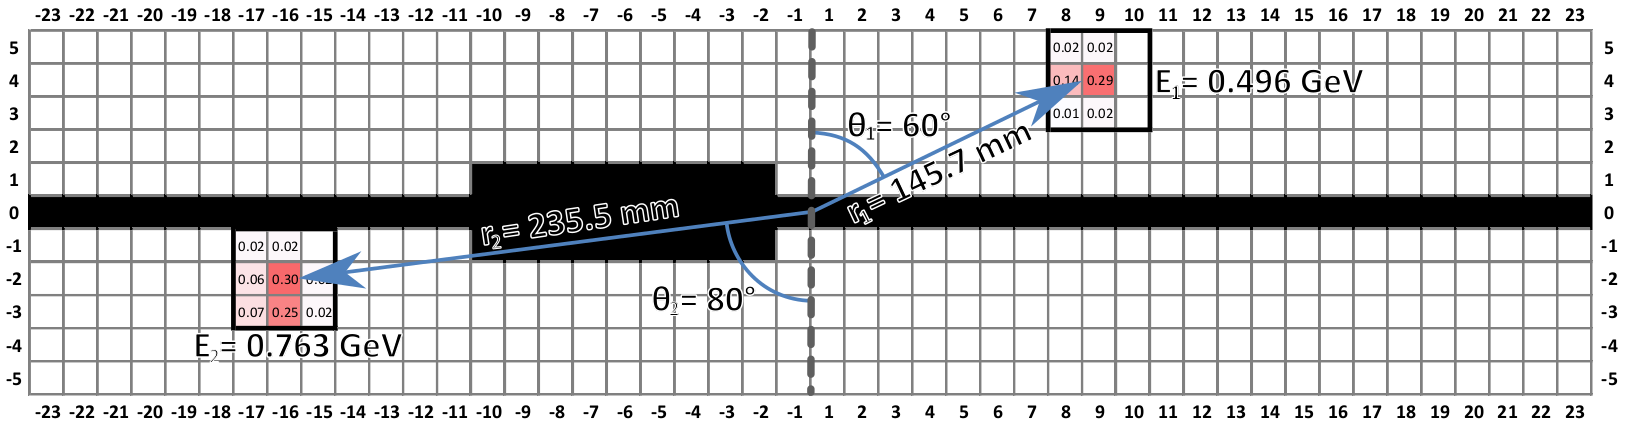
\includegraphics[width=\textwidth]{figures/hps/experiment/skmccarty-thesis-fig-27-pair-trigger-depiction.png}
  \caption{
    Figure 27 of \cite{skmccarty-thesis-2020}. Depiction of an event passing the pair trigger
    in the 2016 data collection run. This depiction also displays the variables used in order
    to evaluate events and make the trigger decision.
  }
  \label{fig:hps-pair-trigger-depiction}
\end{figure}
